\chapter{Implementation}


\section{Implementation Language Choice}

The compiler will be implemented using the Haskell programming language.

During complication the need to traverse trees usually occurs quite
often. Functional languages like Haskell are suited to this task 
due to features such as pattern matching and tail-end recursive optimisation 
which make traversing trees efficient and simple to implement.

The Glasgow Haskell Compiler is available for most platforms, most importantly for Windows, OSX and Linux 
on x86 architectures. This allows the compiler to be portable across these platforms provided the libraries 
used to build the compiler are portable.

Haskell has support for algebraic datatypes, these makes Abstract Syntax Trees
simpler to implement. For example the AST for a very simple expression
can be represented as follows:

\begin{lstlisting}[style=myHaskell]

    data Expression =
          Add Expression Expression
        | Negate Expression 
        | Const Integer

\end{lstlisting}

The equivalent in an Imperative/OOP language (in this case Java)
would be the following:

\begin{lstlisting}[style=myJava]

abstract Class Expression {}

class Add extends Expression {
    public Expression left;
    public Expression right;
    public Add(Expression l, Expression r) {
        left = l;
        right = r;    
    } 
}

class Negate extends Expression {
    public Expression expr;
    public Negate(Expression e) {
        expr = e;    
    }
} 

class Const extends Expression {
    public int value;
    public Const(int v) {
        value = v;
    }
}       

\end{lstlisting}

The Haskell version is much clearer on the structure of the tree, and takes much
less code to implement. 

It is also to easily extend Haskell datatypes to include
custom annotations. For example storing the source code position for parts of expressions 
which is useful for reporting errors to the user.

Due to the pure function nature of Haskell, parts of complilation can easily be performed in parallel.
For example during type checking each GPC function can be type checked in parallel and this can even be subdivided 
further into blocks within functions. For this project speed of compilation is not a major concern, but in the future if compliation ever
needs to be faster then this option is always available.

Haskell also has powerful libraries for parsing source code such as Parsec which is a parser combinator
library. Parsec allows Combinator parsers to be written in the Haskell language itself avoiding the complexity
of integration of different tools and languages\cite{parsec}. 

\section{Tools and Testing}


\subsection{Cabal}

Cabal (Common Architecture for Building Applications and Libraries) is a system for building and
packaging Haskell libraries and programs\cite{cabal}. This system can manage the
project library dependencies, and automatically download and install missing dependencies.
It can also build amd install the compiler on the system, and run unit tests.

\subsection{Testing}

For Unit testing the HUnit library will be used, this can be integrated
with Cabal to easily run all the required unit tests.

One form of testing used for this project is testing each individual component
(e.g. The Parser or the TypeChecker). Each component in the compiler can easily
be uncoupled from one another due to the linear nature of compliation.

Another form of testing is writing GPC source files which should compile, and
GPC files which should fail compilation at a certain stage. The compiler
is then invoked during testing on all of these files to check whether
all the source files which should compile do infact compile with no errors,
and all the source files which should raise an error do not compile.

An upside to this method is that testing this way is flexible in that
tests aren't coupled with the implementation internals of the compiler.
The only way that these test would need to be changed was if the design
of the language itself would need to be changed.

A downside to this method is that without manually checking the errors raised
by the tests that should fail; The source may generate an error which is unrelated
to the error that is being tested. This is why some testing of each internal
component is done alongside this method.

\subsection{Code Coverage}

The Haskell HPC (Haskell Program Coverage) library allows for recording
code coverage over different modules during testing. This can be integrated with
cabal unit testing to automatically generate these results. The usefulness of this
allows for checking which sections of code still need to be tested and assists
in writing further unit tests.


\section{Compiler Structure}
Compilation is split up into multiple stages or "passes",
it is possible to compile in one pass but seperating each 
specific section of compilation allows modularity and decoupling.

\begin{figure}[!htb]
\begin{center}
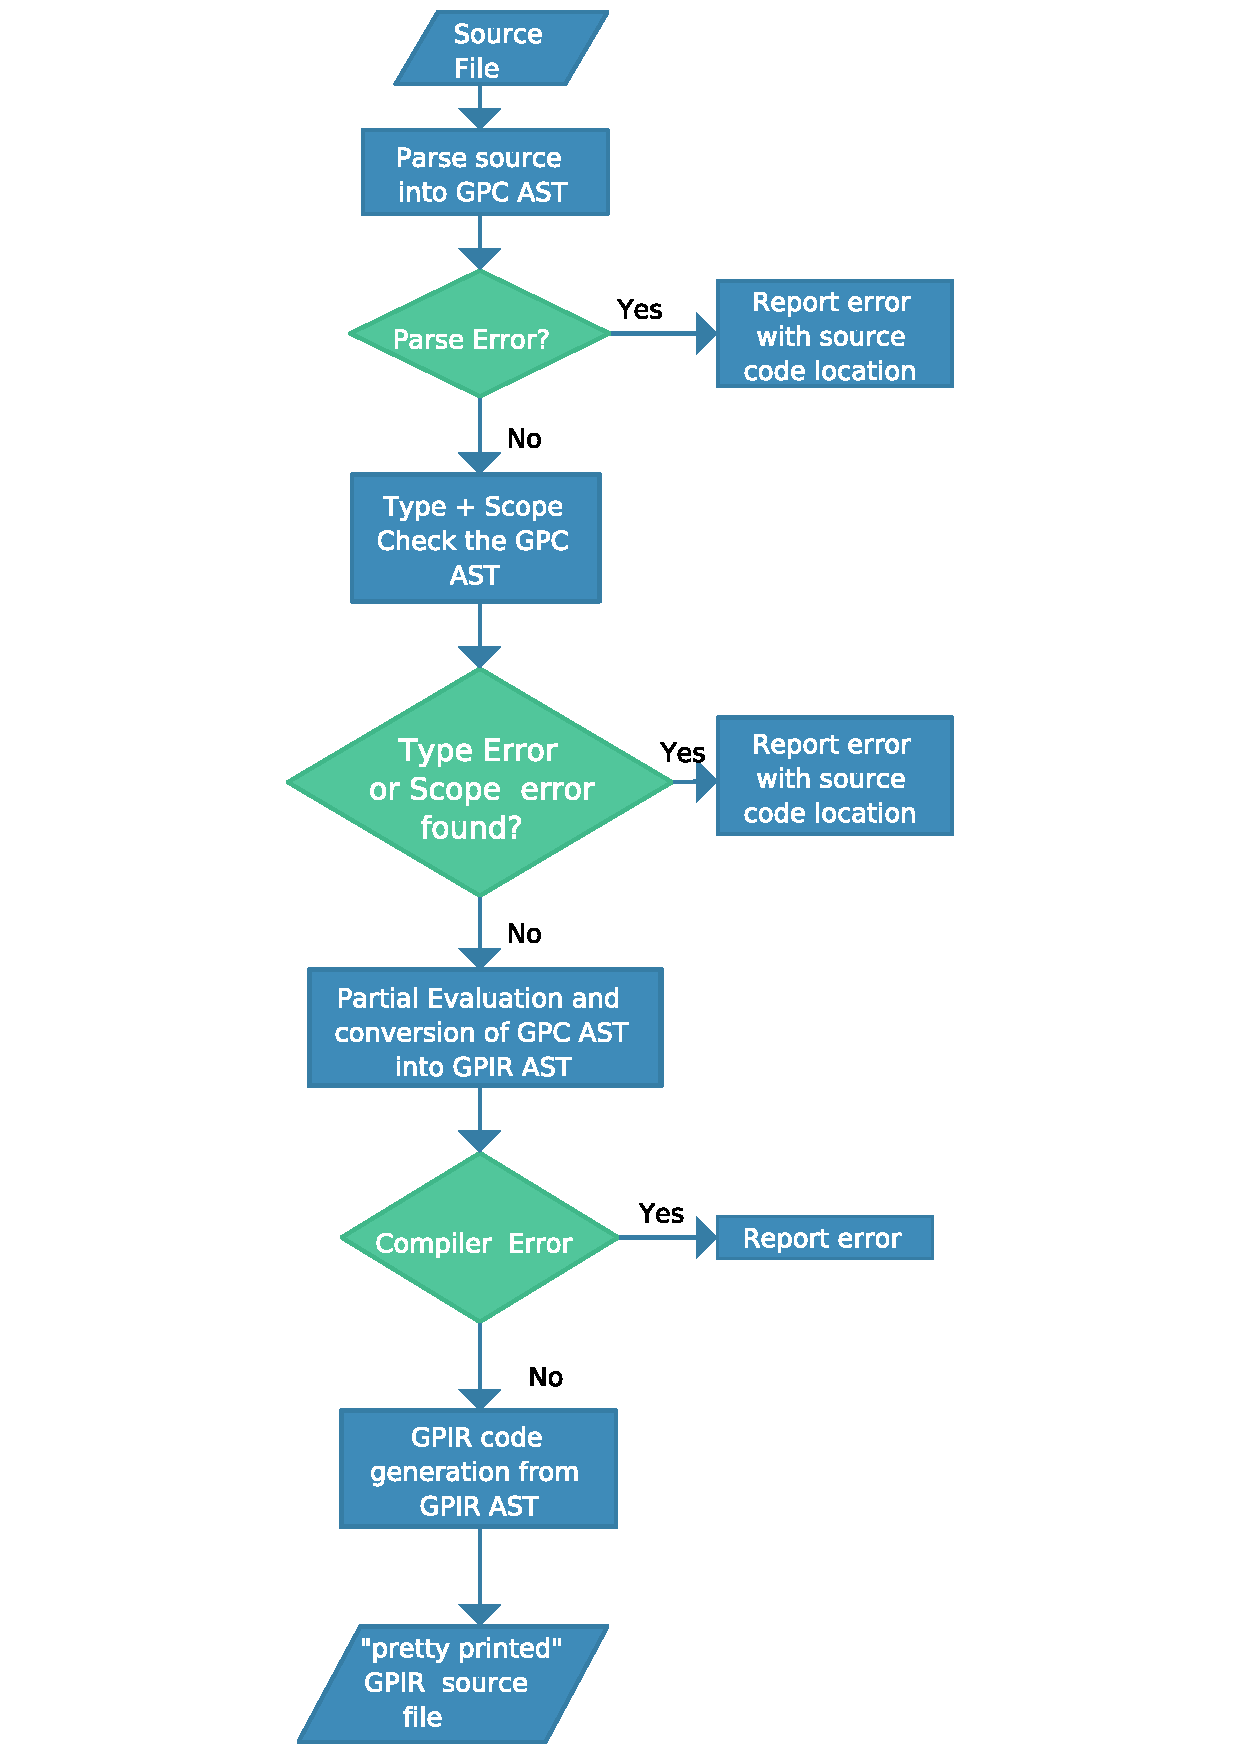
\includegraphics{graphs/Dissertation.pdf}
\caption{Flowchart illustrating the stages of the GPC compiler.}
\end{center}
\end{figure}

    
\section{Parser/Lexer}
The Parsec library combines Parsing and Lexing into one stage.

Given the GPC source file the intention is to parse the file into an AST
to hopefully eventually be transformed into GPIR source code. It's
also useful to store the original source position to provide error information 
during a further compilation stage, to achieve this the source position
info is read from Parsec into an Annotated AST as the tree is being built up.

Parsec does most of the work during this stage, including
providing error messages for "expected" values to be found in source
positions and source position information. Most of the work implementing
this stage is building the parser combinator functions and composing
them together to be able to build the AST.


\section{Type and Scope checking}

During type checking the types of identifiers from the current scope being used in expressions need
to be known. Since the scope needs to be kept track of while type checking it makes reasonable
sense to check for scope errors in the same stage.

The goal of this stage is to ensure that the static typing of the source file
is enforced (e.g. attempting to assign a bool value to a variable of type int should not happen) and,
prevent "logic" errors at compile time (e.g. adding 2 bool values together). Scope checking
is also important as identifiers being used within the program need to be binded to an expression of
some sort, and the "single assignment" rule in the GPC language needs to be enforced.

There are two seperate "types" of scope in a GPC program. The first is the top level scope and the
other is at function level scope. Any scope "further" down from function level scope is itself
a function level scope. During this stage the top level scope will be type and scope checked.
Afterwards each individual function will be type and scope checked.

For checking over top level statements the following Haskell record is used
to keep track of identifier types, objects, and functions encountered:

\begin{lstlisting}[style=myHaskell]
type VarTable = M.Map (Ident SrcPos) (Type SrcPos)
type FunTable = M.Map (Ident SrcPos) (Type SrcPos, [Type SrcPos])
type ObjectTable = M.Map (Ident SrcPos) (Objects SrcPos)

data MainBlock = MainBlock {
    _tlFuncDefs      :: FunTable, -- ^ Function Definitions
    _tlVarTypes      :: VarTable,  -- ^ Top Level Constant variable types
    _objects         :: ObjectTable  -- ^ Table of current Kernel objects declared 
} deriving (Show)
\end{lstlisting}

It needs to be checked that no duplicate functions exist and  no duplicate top level variables exist,
Once all top level statements have been checked, all functions in scope stored, 
all top level variables stored, and all variables stored. Each individual function
can be checked.

A slightly different stucture is needed to type check functions.

At anytime it is needed to be known what variables that are currently in scope, their types,
what functions are avilable to call, their argument types, and return types. Also the
objects which are available to call methods on, and the current function the type checker
is in at any point.

These values can be stored using the following Haskell record: 

\begin{lstlisting}[style=myHaskell]

data CodeBlock = CodeBlock {
    _currentFun :: Ident SrcPos, -- ^ Name of Function block is in
    _funcDefs   :: FunTable, -- ^ Function names and return/argument types
    _prevVars   :: VarTable, -- ^ Identifiers visible in current scope with types
    _curVars    :: VarTable  -- ^ Identifiers declared in current scope
} deriving (Show)


\end{lstlisting}

When a function is being type check a new CodeBlock instance needs to be
created from a MainBlock instance, as some of the top level information is needed.
The details of the function that is being entered is stored in \texttt{\_currentFun}, 
details of all available functions stored in \texttt{\_funcDefs}, and store all
top level variable in \texttt{\_prevVars}. \texttt{\_curVars} is left as an empty map as the
type checking of the function hasn't begun yet. Top level objects are also
stored in \texttt{\_curVars} as an "object" variable type.

Whenever a new scope is encountered by either calling a function, or entering a seq/par block;
A new CodeBlock structure is created using the current structure. The new \texttt{\_curVars}
is set to the empty map as no variables have been encountered yet, the \texttt{\_funcDefs}
are copied as all functions are on the top level so they don't change. The \texttt{\_currentFun}
is copied if entering a block, otherwise if entering a function the function name
and source position are copied. 

The value of the new \texttt{\_prevVars} is a little more complicated to work out.
Any key-value pairs in the current \texttt{\_curVars} are stored plus any key-value pairs in the 
current \texttt{\_prevVars} in which the key isn't present in the current 
set of \texttt{\_curVars} keys. This is because
the identifiers in \texttt{\_curVars} scope are visible over the identifiers with
the same name in \texttt{\_prevScope}. Haskell's union operation on maps
discards the key-value pairs in the second map for keys that are
present in the first map, so this is trivial to implement.

When type checking a function, every statement in the function is type checked
as well as the type of the return statement. For every statement,
every expression within the statement is type checked. This is implemented by traversing
the Statement AST and checking the scopes of identifiers as well as expected types
against actual types.

Objects which are declared are not checked to see if they actually exist. Neither
are method calls which means the argument types and return types when calling them
cannot be determined at compile time. This is due to the fact Objects are instantiated from
C++ classes. The C++ class of the object would need to be checked for 
methods available as well as argument and return types. 
This is already implemented in the GPRM, so an error will occur further down to compile "chain" or during
runtime.

If a type or scope error is encountered, an error message determining the type of error,
and the source position of the error is returned. Otherwise an empty tuple is returned.
When type and scope checking the original AST doesn't need to be modified, only verified
that it follows the type and scope rules of the language.


\section{Interpreting}

The goal of this stage is to run through the execution path the GPIR code
will take from the entry function, and partially evaluate the code as much
as possible while generating the GPIR AST.

Just before interpreting the GPC AST is transformed slightly into a similar AST
with a couple of differences. One is that annotations are not present (since source position information
is not needed anymore), and type information is stripped (since the program has been proven to 
not have any type errors), also objects in the top level scope are stripped. (Since scope checking
proved that all methods are called on objects that exist, and whenever a method is called, the
name of the object is part of the call).

Initially the values of all top level assignment statements need to be stored
as constants before executing, as well as the details for every function.

While interpreting a state is needed to determine actions taken
during certain sections, as well as to evaluate expressions.
The following Haskell record is used:

\begin{lstlisting}[style=myHaskell]

type ConstVarTable = M.Map Ident Literal
type FunTable = M.Map Ident ([Ident], BlockStmt)
type VarRegTable = M.Map Ident Integer

-- ^ Current State of the Block we are currently in
data CodeGen = CodeGen {
   _funTable    :: FunTable,  -- ^ Store symbol tree for functions
   _constTable  :: ConstVarTable, -- ^ Store constants in scope
   _varId       :: Integer, -- ^ Current variable id for mapping to registers
   _varRegTable :: VarRegTable, -- ^ maps variable identifier
   _threadCount :: Integer, -- ^ Current thread number to map
   _maxThreads  :: Integer,  -- ^ Maximum number of threads
   _seqBlock    :: Bool, -- ^ Whether or not current block is sequential
   _isReturning :: Bool -- ^ Whether the state of the current block is in a return
}

\end{lstlisting}


\subsection{Registers}
Values which can be fully evaluated at compile time can be subsituted into the
GPIR code with their literal value when they are used.

For example:

\begin{center}{\textbf{GPC Code}}
\end{center}

\begin{lstlisting}[style=myGPC, frame=single]
seq {
    int x = 4 * 5;
    obj.m1();
    obj.m2(x + 3);
}
\end{lstlisting}

\begin{center}{\textbf{Compiled down to GPIR code}}
\end{center}

\begin{lstlisting}[style=myGPIR, frame=single]
seq (
     '(obj.m1[0]) 
     '(obj.m2[0] '23)
)
\end{lstlisting}

The value of \texttt{x} is able to be calculated to be 20, so whenever
\texttt{x} is used in the scope it can simply be replaced with the literal \texttt{20}.

However, some variables will not be able to be fully evaluated at compile time.
So results will have to be written to GPIR registers.

For example:

\begin{center}{\textbf{GPC Code}}
\end{center}
\begin{lstlisting}[style=myGPC, frame=single]
seq {
    int x = obj.m1();
    obj.m2(x);
}
\end{lstlisting}

\begin{center}{\textbf{Compiled down to GPIR Code}}
\end{center}
\begin{lstlisting}[style=myGPIR, frame=single]
seq (
     '(register.write[0] '1 'obj.m1[0]) 
     '(obj.m2[0] (register.read[0] '1))
)
\end{lstlisting}

The value of \texttt{x} can't be known at compile time so it is written into register \texttt{1},
and then read from the same register when it is needed.

During interpreting, there needs to be no conflict between registers (e.g. if a value
is stored in register 1 that will need to be used later, register 1 cannot be written to
until that value is out of scope). There's no hard limit on registers so a simple
method of just incrementing the register count every time a value needs to be stored
is implemented, although this may possibly cause a lot of unecessary memory usage.

\texttt{\_varRegTable} is used to store the mappings of variable names to register numbers. 
Conflicts between variables with the same name in different scopes is not a problem,
as the register table in the inner block is thrown away once the scope is left.

\subsection{Sequential And Parallel Block Differences}
A sequential block translates to something different in GPIR than a parallel block.

For example, these two snippets compile to different GPIR code despite
the blocks containing the same code:\\


\begin{minipage}{.48\textwidth}
\center \textbf{GPC Parallel}
\begin{lstlisting}[style=myGPC, frame=single]
par {
    obj.m1();
    obj.m2();
}
\end{lstlisting}

\center \textbf{GPIR Parallel}
\begin{lstlisting}[style=myGPIR, frame=single]
(par obj.m1[0] obj.m2[1])
\end{lstlisting}
\end{minipage}
\hfill
%
%
\begin{minipage}{.48\textwidth}
\center \textbf{GPC Sequential}
\begin{lstlisting}[style=myGPC, frame=single]
seq {
    obj.m1();
    obj.m2();
}
\end{lstlisting}

\center \textbf{GPIR Sequential}
\begin{lstlisting}[style=myGPIR, frame=single]
(seq `obj.m1[0] `obj.m2[1])
\end{lstlisting}
\end{minipage}
 
Sequential statements need to be quoted, which is why the record contains
the \texttt{\_seqBlock} flag, so the interpreter can generate the correct GPIR code.

\subsection{Thread Mapping}
Each task in the GPRM must be mapped to a thread. There is a function
in the Interpreter called \texttt{getThread} which calculates what the next thread 
number should be to map the task to based on the current block state.

Currently this function uses a simple incremental scheme and rolls around
modulo style after the max number of threads have been specified. The compiler
attempts to work out the maximum number of cores on the machine if a thread
number isn't given, and uses this number to determine the max number of threads.

If a different scheme is needed the contents of the function will need to be changed,
a possible future improvement may be to pass a function to the interpreter when passing
it the AST to determine the counting scheme. This would allow for multiple different schemes
to be chosen and possibly tuned depending on the type of application.


\subsection{Branching}
When encountering an if statement the interpreter must be able to evaluate the condition and generate a
true or false value. The interpreter will only evaluate the statement within the if statement
if the condition is true. In the case of an if-else statement either the first statement will
be evaluated or the else statement depending on the value of the condition.


\subsection{Returning From Functions}
Performing a return is a bit tricky. 

Some pre-evaluation is needed  on blocks of statements when entering a 
new block. if a return statement is
in the current block of statements (not counting sub-blocks) then
any statements after that are "removed", and when a return statement
is found, it is evaluated as the return expression.
What this means is that once the return is met, the interpreter
"returns" back to the code which executed the previous scope.

There are also two different scenarios when performing a return.

If the interpreter is in a function at the top level of the function:
Returning is simple in this case, all that is needed to be done is
going to the previous scope.

If the interpreter is nested within one or more blocks in a function:
Returning in this case involves going up multiple times until the interpreter
is out of the scope of the current function.

To deal with these situations a "boilerplate" function is used. This function
is called whenever an inner-scope needs to be interpreted. It
takes a boolean value which determines if the current block scope is at
the "top" of a function, gets the current state and then interprets the block.
Once the interpreter returns from interpreting the inner block, the "\_isReturning"
flag is checked on the returned state. If it is set, and the scope
of the current block is at the top of a function, then the "\_isReturning" flag
is then set for the current block.
 
When the "\_isReturning" flag is set for a block, the evaluator will not evaluate
any further statements in the current block. This allows for propogation of a "return"
up the block states until the current function is exited.


\subsection{Interpreting Functions}
When a function is called, each argument identifier in scope
is replaced by the the expression which was supplied to the function.
Then each statement in the function is evaluated.

\begin{lstlisting}[style=myGPC]

void fun(int a) {
    obj.m1(a);
    seq {
        int a = 10;
        obj.m3(a);
    }    
}

fun(5 * 4);

\end{lstlisting}

In this example when evaluating the functional call with the argument \texttt{(5 * 4)},
every \texttt{a} which is the same instance as the one in the function arguments
is replaced by the expression \texttt{(5 * 4)}. The nested \texttt{a} is not the same
instance and is not substituted.


\subsection{For Loop Evaluation}

For evaluating and unrolling for loops each loop statement needs to be evaluated
until the loop variable doesn't satisfy the condition. 

\begin{itemize}
\item The iterate function in Haskell can be used to infinitely apply the afterthought function
of the loop to generate loop variable values for each iteration.

\item Then values are taken from this list and are applied to the loops condition until
one fails. This creates a list of loop variables values for all iterations. 

\item This value list is then mapped to the statements in the loop body replacing any instance
of the loop variable. This unrolls the loop.

\item Then each statement is then evaluated. 
\end{itemize}


It is also possible to detect cases of infinite loops based on the loop variable, 
the conditional, and afterthought statements, before attempting to unroll the loop.

For example the following for loop will loop infinitely (Ignorning overflow of integers, which is undefined in most C/C++ standards).
\begin{lstlisting}[style=myGPC]
for (int i = 0; i < -1; i++) {
    obj.m1(i);
}
\end{lstlisting}


\subsection{Partial Expression Evaluation}
\label{sub:partial}

There are two parts needed to evaluate an expression:

\begin{itemize}
    \item Replacement - All identifiers in the expression which have a value in the constant table are
          replaced with the respective constant value.

    \item Reduction - Attempt to evaluate as much of the replaced expression as possible

\end{itemize}

Replacement is trivial, using the constant table for the current scope the
expression AST is recursively travelled and any instances of identifiers
in the constant table are replaced.


Reduction is a bit more complex, it involves attempting to apply the binary
and unary operations to their respective expressions. Expressions can be
represented in a binary expression tree. Binary operators are contained in
the inner nodes with 2 children, unary operators contained in the inner
nodes with 1 child. Leaf nodes contain literal values and variables.

For example the expression \texttt{5 * 3 - 2 + \textasciitilde2} when read in by the
compiler is represented by the following tree:

\begin{center}
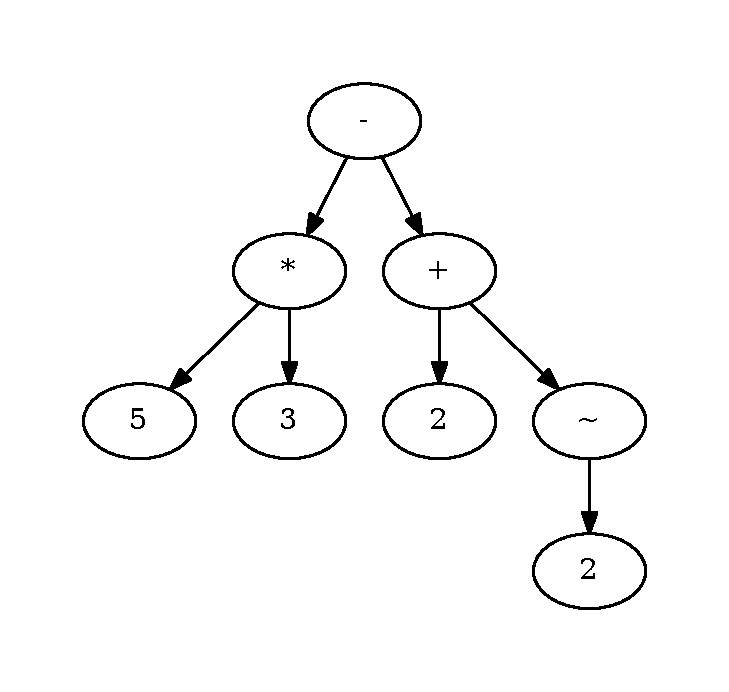
\includegraphics[scale=0.5]{graphs/impleval.pdf}
\end{center}


The tree is evaluated through
postorder traversal. Once two leaf nodes are found the binary operation in the parent node
is attempted to be applied to the two leaf nodes, or if one leaf node is found
with no other node the unary operation in the parent node is applied
to the leaf.  

In the case of a binary operation if both leaf nodes are values which
can be calculated at compile time the expression is evaluated, the two leaf nodes
are removed and the parent node is replaced with the calculated value. If one or
more leaf nodes are values which can only be known at runtime then the expression is
not evaluated and the tree doesn't change. 

In the case of a unary operation if the leaf node is a value which can be calculated
at compile time the expression is evaluated, otherwise the expression is not evaluated
and the tree doesn't change.

However this method isn't optimal when some sub-expressions cannot be
evaluated at compile time. In this case the expression can only be partly evaluated,
but depending on the expression this method can at times reduce the expression
down to an expression which can still be further reduced.
This problem and a possible solution is discussed in Chapter ~\ref{ch:future}.



\section{GPIR Code Generation}

Once the interpreter is completed it should produce the GPIR AST, 
from this AST the goal is to output GPIR source code.
Since the GPIR language is very simple this task is not too difficult.,
It involves recursively travelling the tree, ensuring lists containing task operations
are surrounded by parenthesis, printing quotes when needed, etc.

For this task a "pretty printer" library is used which allows for formatting
the output much easier than manipulating strings. The generated GPIR source code
is saved into a file with the same prefix as the source but with a ".td" (Task Description)
extension.
